\section{Security analysis}
In this assignment, I will examine the security of toll collection point, 
commonly referred to as toll booths. 

\begin{figure}[h]
\centering
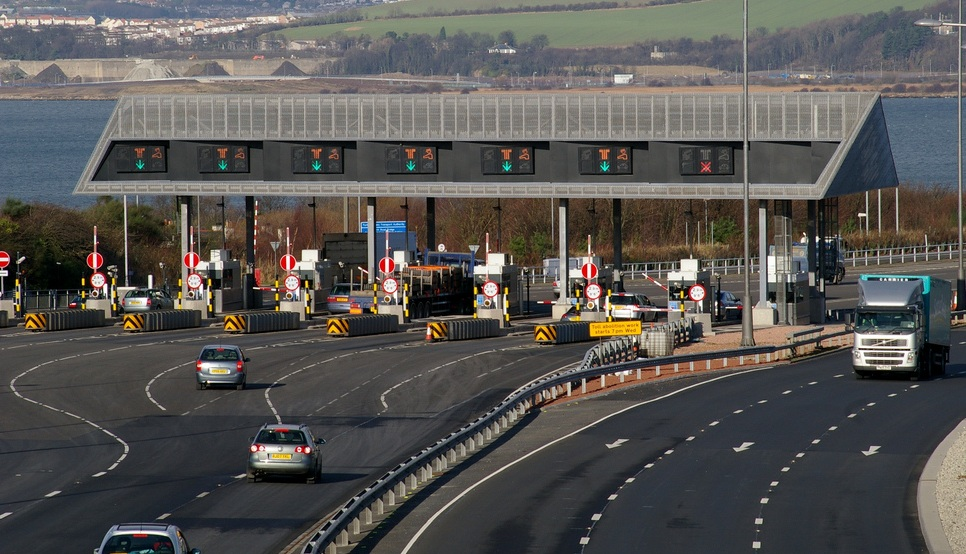
\includegraphics[scale=0.2]{toll_booth}
\caption{A toll booth}
\label{fig:booth}
\end{figure}

Toll booths are usually in place to secure either access to a given road, or
ensure that travellers travelling along the given road pays for distance
travelled. They are also in place between country borders, to keep out unwanted
foreigners.

Historically they have been used by kings and lords, to control roads, either
by sea or by foot, usually in the form of castles at strategic places(ex.
Kronborg).

\subsection{Assets and Security goals}
The main asset in this context is the road or the lands beyond the booth, it 
can be controlled for different reasons, that being security for the traveller,
maintenance of the road or simply limiting access.

Another asset is the actual stand, this is the main enforcing mechanism of the 
system, and is therefore ciritical to its function.

In short the assets are:
\begin{itemize}
\item road/land
\item booth/stand
\end{itemize}

\paragraph{The goal} of the system is to secure that no unwanted traffic is
going through.

\subsection{Adversaries and threats}

\subsection{Weaknesses and defences}

\subsection{Risk analysis}

\subsection{Conclusion}
